\chapter{问题介绍}

\section{量子模型检测中的关键问题}
\begin{itemize}
  \item 可达性分析
  \item 模型检验的挑战
\end{itemize}
% //TODO: add key problem here
\subsection{跃迁系统}
跃迁系统广泛应用于模型检测中待检测系统的建模,其定义为\citep{baier2008principles}:
\begin{equation}
\mathcal{M}=\{S,Act,\rightarrow,I\}
\end{equation}
其中\(S\)为系统状态集合,\(I\)为系统初态集合,因此满足\(I\subseteq S\)。\(Act\)为系统行为集合。\(\rightarrow\)为系统状态转移关系,即\(\rightarrow\subset S\times Act\times S\)。此外还有\(AP\)为描述系统原子命题。L是标记函数,将状态映射为状态满足的原子命题集合。需要验证的属性\(\varphi\)将表述为命题。


系统的有限路径片段\(\pi\)是一个有限状态序列\(s_0,s_1\ldots s_n\)。\(s_i\)满足\(s_{i-1}\overset{a}{\rightarrow}s_i,a\in Act\),对于所有\(0<i\leq n\),其中\(n\geq 0 \)。无限路径片段\(\pi\)是一个无限状态序列\(s_0,s_1\ldots\),使得对于所有\(i>0\),\(s_{i-1} \overset{a}{\rightarrow}  s_i,a\in Act\)。在路径中\(\pi\left[i\right]=s_i,\pi\left[i\right)=s_i\ldots\)。所有以\(s_0\)为开始的路径,构成了路径集合\(Path\left(s_0\right)\)。

\begin{figure}[!htbp]
    \centering
    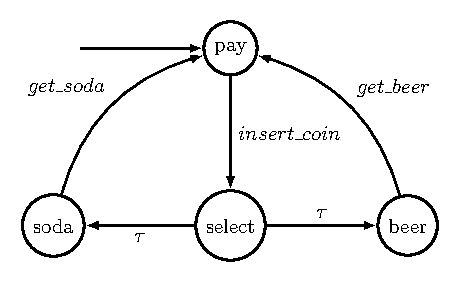
\includegraphics[width=.6\textwidth]{Img/map.pdf}
    \caption{一种简化版的售货机跃迁系统}
    \label{fig:transition-system}
\end{figure}

图\ref{fig:transition-system} 所示的跃迁系统展示了一个简化版的售货机模型。在该模型中,用户投入硬币,进行选择后就可以得到苏打水或者啤酒。在该例子中,系统状态\(S=\{pay,select,soda,beer\}\),系统初态\(I=pay\)。
系统行为\(Act=\{insert\_coin,\tau,get\_soda,get\_beer\}\),其中\(\tau\)表示立即行动符号。转移关系图中已经展示。原子命题可取\(AP=\{paid,drink\}\)。因此\(L\left( pay \right)=\{\varnothing\}\),\(L\left(soda\right)=L\left(beer\right)=\{paid,drink\}\),\(L\left(select\right)=\{paid\}\)。系统的一个路径是\(\pi=pay\ select\ soda\ pay\ selsect\ \ldots\)。此时\(\pi\left[1\right]=slect,\pi\left[1\right)=select\quad soda\quad pay\quad selsect\ldots\)。同时该路径满足\(\pi\in Path\left(pay\right)\)。
量子模型检测的跃迁系统类似。区别在于状态空间用\(\mathcal{H}\),转移关系用酉矩阵。一个量子自动机定义如下:
\begin{align}
    \mathcal{M}=\{\mathcal{H},Act,\{U_\alpha,\alpha\in Act\},\mathcal{H}_0\}
\end{align}
下面介绍模型检测中的使用的时序逻辑。

\subsection{时序逻辑的验证}
在量子模型检测中,与经典模型检测一样使用时序逻辑指定待验证的属性\(\varphi\)。时序逻辑命题的运算符有两类\citep{goranko_2023}。状态命题公式(State formulas):\(\varphi ::=a\left|\exists\varphi\right|\forall \varphi\left|\lnot\varphi\right|\varphi\land\psi\),其中\(a\in AP\)。以及路径命题公式(Path formulas):\(\varphi\Colon=O\varphi|\varphi U\psi\)。给定模型的一个状态为\(s\),路径为\(\pi\),则具体满足条件分别如下:
\begin{itemize}
    \item \(s\models a,iff \L\left(s\right)\models a\)
    \item \(s\models\exists\varphi,iff\ \pi\models\varphi\)对一些\(\pi\in Path\left(s\right)\)
    \item \(s\models\forall\varphi,iff\ \pi\models\varphi\)对所有\(π\in Paths\)
    \item \(s\models\lnot\varphi,iff\ s\nvDash\varphi\)
    \item \(s\models\varphi\land\psi,iff\ s\models\varphi\ and\ s\models\psi\)
    \item \(\pi\models O\varphi,iff\ \pi\left[1\right]\models\varphi\)
    \item \(\pi\models\varphi U\psi,iff\ \exists j\geq0\).\(\pi\left[j\right)\models\psi\) 同时对所有\(0\le i<j\)有\(\pi\left[i\right)\models\varphi\)
\end{itemize}


图\ref{fig:path-formula-basic} 展示了两种路径命题公式的直观示意图。


\begin{figure}[!htbp]
    \centering
    \begin{subfigure}[b]{0.8\textwidth}
        \centering
        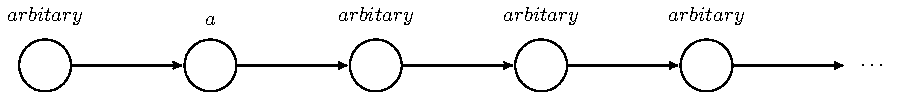
\includegraphics[width=\textwidth]{Img/path_for_Oa.pdf}
    \end{subfigure}
    \\
    \begin{subfigure}{0.8\textwidth}
        \centering
        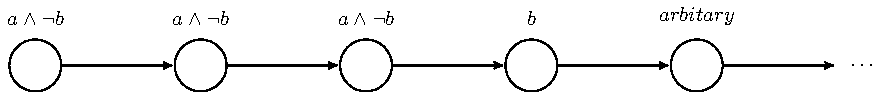
\includegraphics[width=\textwidth]{Img/path_for_aUb.pdf}
    \end{subfigure}
    \caption{路径命题公式$\pi\models O a $与 $\pi\models a U b$的图示}
    \label{fig:path-formula-basic}
\end{figure}
在模型检测中,有三类比较重要的可达性问题,分别是可达性、持续可达性以及重复可达性。过程中主要涉及以下路径命题公式:\(\lozenge\) 表示最终(eventually),\(\square\)表示总是(always),\(\lozenge\square\)表示总是最终(always eventually),\(\square\lozenge\)表示最终总是(eventually always)。其中\(\lozenge\)和\(\square\)具体定义为:
\begin{itemize}
    \item \(\lozenge\varphi\overset{\text{def} }{=} \text{True}U\varphi\)
    \item \(\square\varphi\overset{\text{def} }{=} \neg\lozenge\neg\varphi\)
\end{itemize}
图\ref{fig:path-formula}展示了这两种基本路径命题公式的直观示意图。
\begin{figure}[!htbp]
    \centering
    \begin{subfigure}[b]{0.8\textwidth}
        \centering
        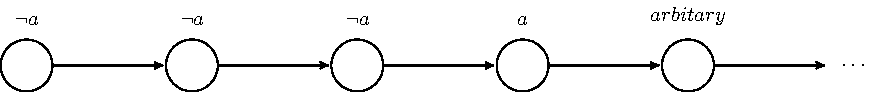
\includegraphics[width=\textwidth]{Img/path_for_Dia.pdf}
    \end{subfigure}
    \\
    \begin{subfigure}{0.8\textwidth}
        \centering
        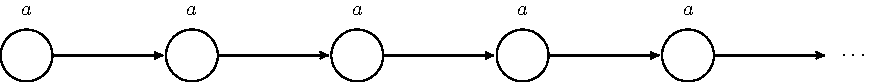
\includegraphics[width=\textwidth]{Img/path_for_SQa.pdf}
    \end{subfigure}
    \caption{路命题公式$\pi\models\lozenge a$与 $\pi\models\square a$的图示}
    \label{fig:path-formula}
\end{figure}

具体的可满足条件为:
\begin{itemize}
    \item \(\pi\models\lozenge\varphi,iff\exists j\ge0.\pi[j)\models\varphi\)
    \item \(\pi\models\square\varphi,iff\forall j\ge 0.\pi[j)\models\varphi\)
    \item \(\pi\models\lozenge\square\varphi,iff\exists i\ge 0.\forall j\ge i,\pi[j)\models\varphi\)
    \item \(\pi\models\square\lozenge\varphi,iff\forall i\ge 0.\exists j\ge i,\pi[j)\models\varphi\)
\end{itemize}
基于此三种可达性问题定义分别如下:
\begin{itemize}
    \item 可达性:\( Pr^{\mathcal{M}}(s \models \lozenge G) = Pr^M(\pi \models \lozenge G : \pi \in \text{Paths}(s))\)
    \item 持续可达性:\( Pr^{\mathcal{M}}(s \models \lozenge \square G) = Pr^M(\pi \models \lozenge \square G : \pi \in \text{Paths}(s))\)
    \item 重复可达性:\( Pr^{\mathcal{M}}(s \models\square \lozenge G) = Pr^M(\pi \models \square\lozenge G : \pi \in \text{Paths}(s))\)
\end{itemize}

\section{TDD在量子模型检测中的应用}

\section{研究问题的现实意义}
% \begin{itemize}
%   \item QDA方面的验证
% \end{itemize}
% //TODO: add usage here
